% Title : hw
% Author: Bhishan Poudel
% Date  : Oct 31, 2015

\documentclass[11pt,a4paper,english]{article}
\usepackage{babel}
\usepackage{amsmath}
\usepackage{amssymb}
\usepackage{graphicx}
\usepackage{textcomp}
\usepackage{fixltx2e}
\usepackage[usenames,dvipsnames,svgnames,table]{xcolor}
\graphicspath{ {figures/} } % Put figures inside this directory and use pdf

% for listing
\usepackage{enumitem}
\usepackage[ampersand]{easylist}
\ListProperties(Hide=100, Hang=true, Progressive=3ex, Style*=-- ,
Style2*=$\bullet$ ,Style3*=$\circ$ ,Style4*=\tiny$\blacksquare$ )    % for easylist
\newcommand{\begl}{\begin{easylist}}
\newcommand{\eegl}{\end{easylist}}

% for hyperlink
\usepackage{hyperref}             % for hyperlink
\hypersetup{
    colorlinks=true,
    linkcolor=blue,
    filecolor=magenta,
    urlcolor=cyan,
    bookmarks=true
    }


% Creating Title for the assessment
\title{Homework 9: Monte Carlo Application}
\author{Bhishan Poudel}
\date{Oct 31,2015}

% to avoid indentation in paragraphs
\usepackage[parfill]{parskip}

% begin of document
\begin{document}
\maketitle
\tableofcontents
\listoffigures
\clearpage

%%%%%%%%%%%%%%%%%%%%%%%%%%%%%%%%%%%%%%%%%%%%%%%%%%%%%%%%%%%%%%%%%%%%%%%%%%%%%%%%%%%%%%%%%%%%%%%%%%%%%

\section{Question 1: Random Sequences }

This is a figure.
	\begin{figure}[h!]
	\centering
	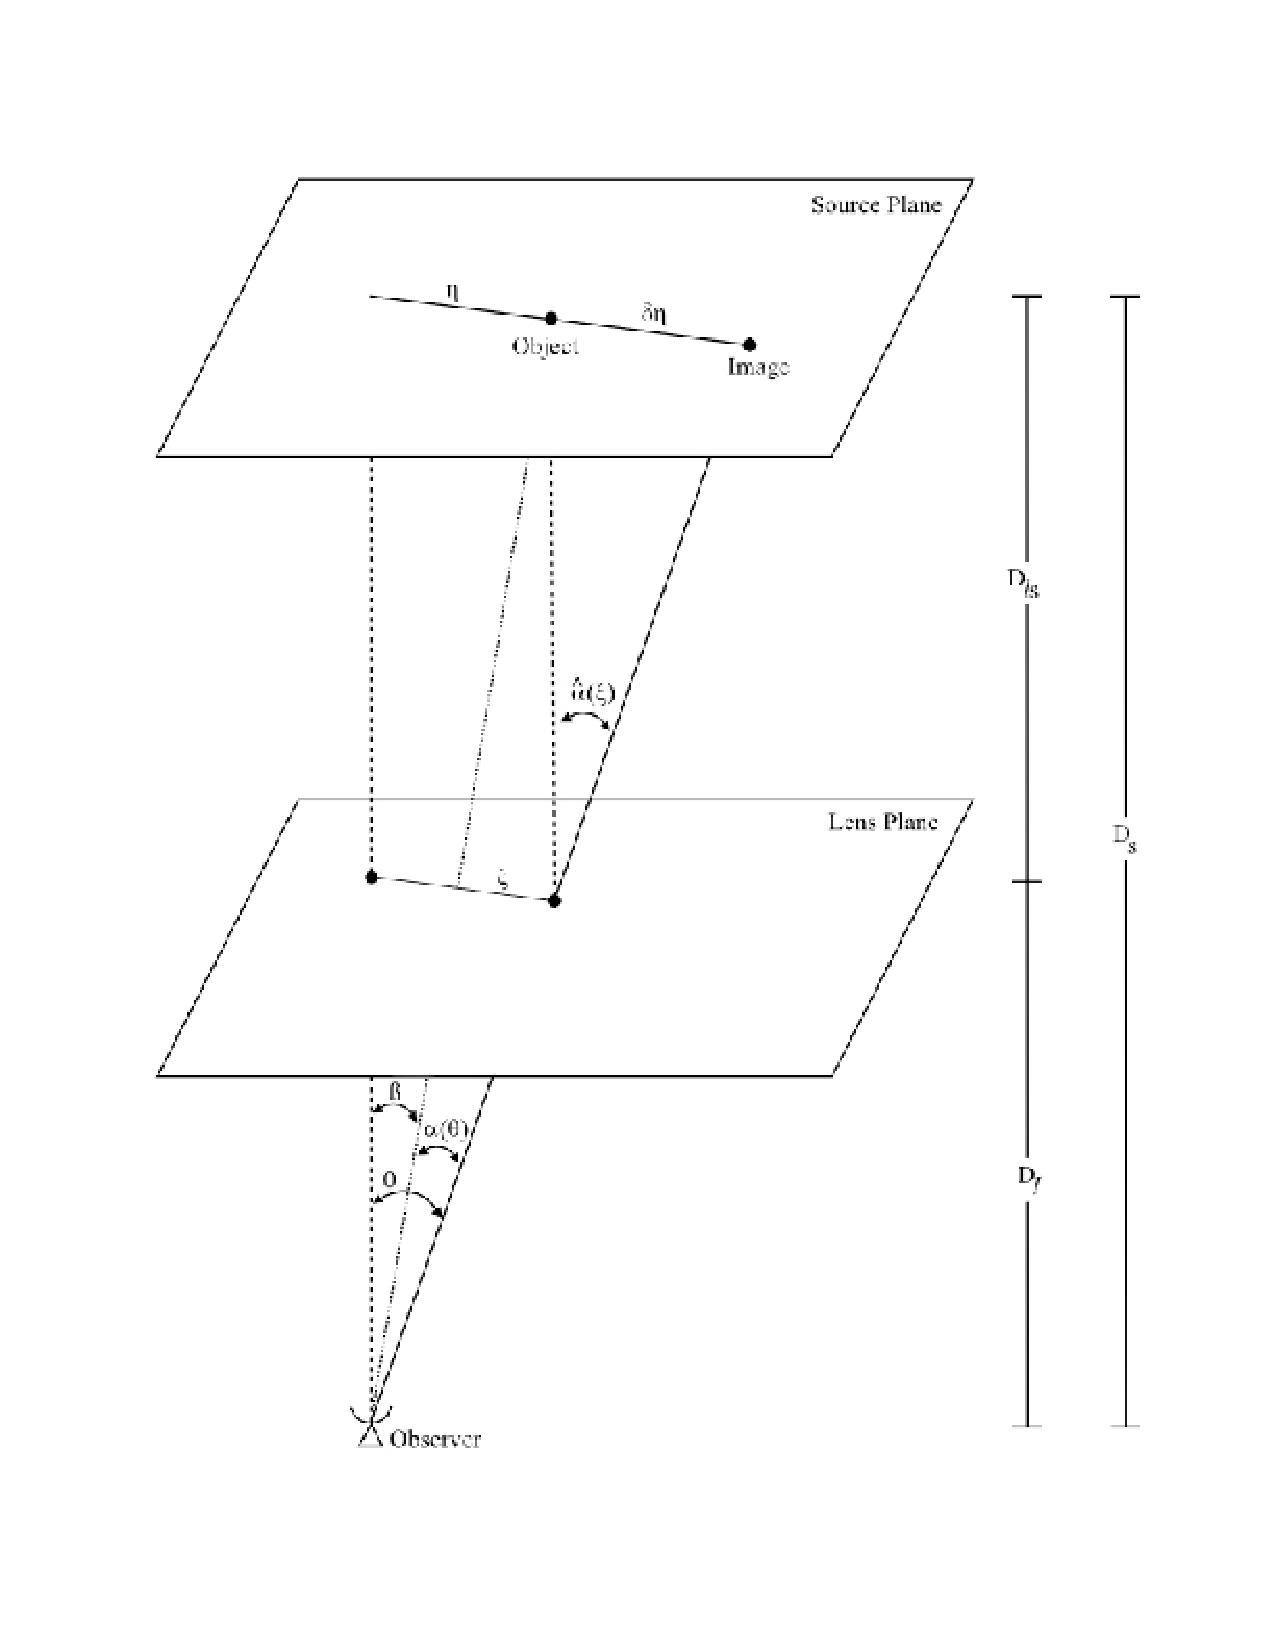
\includegraphics [scale=0.6,angle=0]{lensing}
	\caption{ }
	\end{figure}



\end{document}
